% Created 2021-09-23 Thu 17:56
% Intended LaTeX compiler: pdflatex
\documentclass{article}
\usepackage[utf8]{inputenc}
\usepackage[T1]{fontenc}
\usepackage{graphicx}
\usepackage{grffile}
\usepackage{longtable}
\usepackage{wrapfig}
\usepackage{rotating}
\usepackage[normalem]{ulem}
\usepackage{amsmath}
\usepackage{textcomp}
\usepackage{amssymb}
\usepackage{capt-of}
\usepackage{hyperref}

\usepackage[a4paper,left=0.5in,right=0.5in,top=0.5in,bottom=1in]{geometry}
\usepackage{float}
\usepackage{enumerate}
\DeclareUnicodeCharacter{2212}{-}
\setcounter{secnumdepth}{0}
\author{Tzong Lin Chua}
\date{\today}
\title{EE4C10 Analog Circuit Design Fundamentals\\\medskip
\large Homework Assignment II }
\hypersetup{
 pdfauthor={Tzong Lin Chua},
 pdftitle={EE4C10 Analog Circuit Design Fundamentals},
 pdfkeywords={},
 pdfsubject={},
 pdfcreator={Emacs 27.1 (Org mode 9.5)}, 
 pdflang={English}}
\begin{document}

\maketitle
\tableofcontents


\section{Problem 1}
\label{sec:org82972da}
\begin{enumerate}[(a)]
\item Overdrive voltage, V\textsubscript{gt}, for:
\begin{enumerate}[1.]
\item M1
\begin{equation*}
\begin{aligned}
I_{D1} &= \frac{\mu_{n}C_{OX}}{2}(\frac{W}{L})_{1}(V_{GS_{1}} - V_{TH_{1}})^2(1 + \lambda_{1}V_{DS_{1}}) \\
I_{D1} &\approx \frac{\mu_{n}C_{OX}}{2}(\frac{W}{L})_{1}(V_{gt_{1}})^2 \\
V_{gt_{1}} &\approx \sqrt{\frac{2 I_{D_{1}}}{\mu_{n}C_{OX}}(\frac{L}{W})_{1}} \\
\\
V_{gt_{1}} &\approx 109.11 mV
\end{aligned}
\end{equation*}

\item M2
\begin{equation*}
\begin{aligned}
V_{gt_{2}} &\approx \sqrt{\frac{2 I_{D_{2}}}{\mu_{p}C_{OX}}(\frac{L}{W})_{2}} \\
\\
V_{gt_{2}} &\approx 377.96 mV
\end{aligned}
\end{equation*}
\end{enumerate}

\item Small-signal gain

\begin{equation*}
\begin{aligned}
g_{m1}V_{in} &= \frac{-V_{out}}{r_{o1}//r_{o2}} \\
\frac{V_{out}}{V_{in}} &= -g_{m1}(r_{o1}//r_{o2}) \\
\\
g_{m1} &= \mu_{n}C_{OX} (\frac{W}{L})_{1} V_{gt_1} \\
&= 4.582 mS \\
\\
r_{o1} &= \frac{1}{I_{D1}\lambda_{n}} \\
&= 20 k\Omega \\
\\
r_{o2} &= \frac{1}{I_{D2}\lambda_{p}} \\
&= 40 k\Omega \\
\\
\frac{V_{out}}{V_{in}} &\approx -61.09 \\
\end{aligned}
\end{equation*}

\item V\textsubscript{out} output swing

For M\textsubscript{1} to be in saturation,
\begin{equation*}
\begin{aligned}
V_{DS1} &\geq V_{gt1}\\
V_{out} &\geq 0.109 V
\end{aligned}
\end{equation*}

For M\textsubscript{2} to be in saturation,
\begin{equation*}
\begin{aligned}
V_{DS2} &\geq V_{gt2} \\
V_{DD} - V_{out} &\geq 0.377 V \\
V_{out} &\leq 3.3 V - 0.377 V \\
V_{out} &\leq 2.923 V \\
\end{aligned}
\end{equation*}

Swing of V\textsubscript{out},
\begin{equation*}
\begin{aligned}
0.109 V &< V_{out} < 2.923 V \\
\\
V_{out, pp} &= 2.923 V - 0.109 V \\
&= 2.814 V
\end{aligned}
\end{equation*}

\item 
\end{enumerate}

\section{Problem 2}
\label{sec:orgb9789dc}
\begin{enumerate}[(a)]
\item For M1 to be 100mV from triode,
\begin{equation*}
\begin{aligned}
V_{DS1} &= V_{GS1} - V_{TH,N} + 100mV \\
X &= V_{in} - V_{TH,N} + 100mV \\
\end{aligned}
\end{equation*}
V\textsubscript{in} for M1 to be in saturation with I\textsubscript{D1} of 0.35 mA,
\begin{equation*}
\begin{aligned}
I_{D1} &= \frac{\mu_{n}C_{OX}}{2}(\frac{W}{L})_{1}(V_{GS1} - V_{TH,N})^2 \\
I_{D1} &= \frac{\mu_{n}C_{OX}}{2}(\frac{W}{L})_{1}(V_{in} - V_{TH,N})^2 \\
V_{in} &= \sqrt{\frac{2I_{D1}}{\mu_{n}C_{OX}}(\frac{L}{W})_{1}} + V_{TH,N} \\
&= 0.653 V \\
\\
X &= \sqrt{\frac{2I_{D1}}{\mu_{n}C_{OX}}(\frac{L}{W})_{1}} + 100mV \\
&\approx 0.253 V
\end{aligned}
\end{equation*}
V\textsubscript{b} for M2 to be in saturation with I\textsubscript{D2} of 0.35 mA,
\begin{equation*}
\begin{aligned}
I_{D2} &= \frac{\mu_{n}C_{OX}}{2}(\frac{W}{L})_{2}(V_{GS2} - V_{TH,N})^2 \\
I_{D2} &= \frac{\mu_{n}C_{OX}}{2}(\frac{W}{L})_{2}(V_{b} - X - V_{TH,N})^2 \\
V_{b} &= \sqrt{\frac{2I_{D2}}{\mu_{n}C_{OX}}(\frac{L}{W})_{2}} + X + V_{TH,N} \\
&\approx 0.906 V

\end{aligned}
\end{equation*}

\item Small-signal gain

\begin{equation*}
\begin{aligned}
G_{m} &= \frac{g_{m1}(g_{m2}r_{o1}r_{o2} + r_{o1})}{g_{m2}r_{o1}r_{o2} + r_{o1} + r_{o2}} \\
&\approx g_{m1}
\end{aligned}
\end{equation*}
\begin{equation*}
\begin{aligned}
R_{out} &= (g_{m2}r_{o1}r_{o2} + r_{o1} + r_{o2}) // R_{d} \\
\end{aligned}
\end{equation*}

Small-signal gain,
\begin{equation*}
\begin{aligned}
\frac{V_{out}}{V_{in}} &= -G_{m}R_{out} \\
&= -g_{m1}[(g_{m2}r_{o1}r_{o2} + r_{o1} + r_{o2}) // R_{d}] \\
\\
g_{m1} &= \mu_{n}C_{OX} (\frac{W}{L})_{1} (V_{GS1} - V_{TH,N}) \\
&= \mu_{n}C_{OX} (\frac{W}{L})_{1} (V_{in} - V_{TH,N}) \\
&= 4.583 mS \\
\\
g_{m2} &= \mu_{n}C_{OX} (\frac{W}{L})_{2} (V_{GS2} - V_{TH,N}) \\
&\approx \mu_{n}C_{OX} (\frac{W}{L})_{2} (V_{b} - X - V_{TH,N}) \\
&= 4.583 mS \\
\\
r_{o1} &= \frac{1}{I_{D1}\lambda_{n}} \\
&= 28.571 k\Omega \\
\\
r_{o2} &= \frac{1}{I_{D2}\lambda_{p}} \\
&= 28.571 k\Omega \\
\\
\frac{V_{out}}{V_{in}} &\approx -22.88 \\
\\
\end{aligned}
\end{equation*}

\item Assume V\textsubscript{b} to be 1.65V,
For M2 to be in saturation,
\begin{equation*}
\begin{aligned}
V_{out} - X &\geq V_{b} - X - V_{TH,N} \\
V_{out} &\geq 1.15 V \\
\end{aligned}
\end{equation*}

When \(I_{D} \geq 0\),
\begin{equation*}
\begin{aligned}
V_{out} &\leq V_{DD} \\
1.15 V \leq V_{out} &\leq 3.3V \\
\\
V_{out,pp} = 2.15V
\end{aligned}
\end{equation*}

\item X\textsubscript{pp}

Gain of X,
\begin{equation*}
\begin{aligned}
\frac{X}{V_{in}} &= \frac{-g_{m1}}{g_{m2} + \frac{1}{r_{o1}} + \frac{1}{r_{o2}}} \\
&\approx \frac{-g_{m1}}{g_{m2}} \\
&\approx -1 \\
\end{aligned}
\end{equation*}
X\textsubscript{pp}
\begin{equation*}
\begin{aligned}
\frac{X}{V_{out}} &= \frac{X}{V_{in}}\frac{V_{in}}{V_{out}} \\
&= \frac{1}{22.88} \\
\\
X_{pp} &= 54.63 mV\\
\end{aligned}
\end{equation*}
\end{enumerate}
\section{Problem 3}
\label{sec:org0495006}
\begin{enumerate}[(a)]
\item Sketch of:
\begin{enumerate}[1.]
\item Output voltage
\begin{figure}[H]
\centering
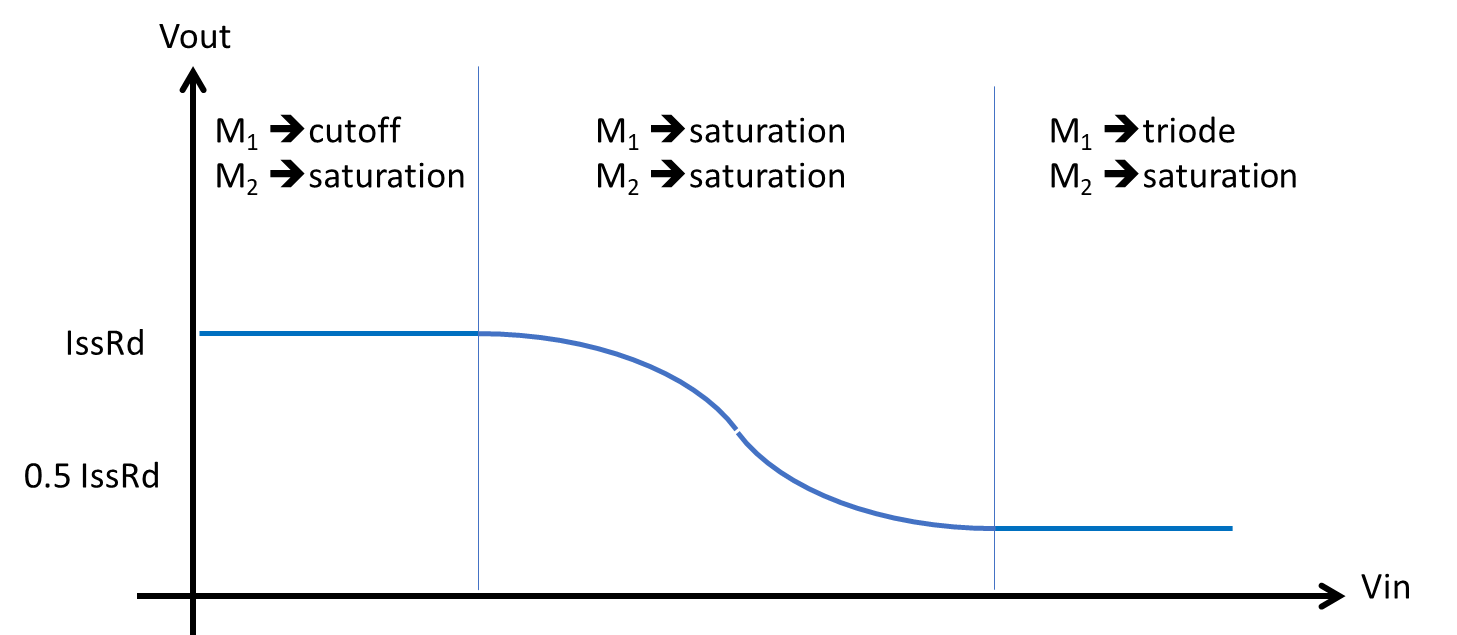
\includegraphics[width=300px]{img/q3/output-voltage-sketch.pdf}
\caption{\label{fig:output-voltage-sketch-q3}Output voltage sketch}
\end{figure}
\item Small-signal gain
\begin{figure}[H]
\centering
\includegraphics[width=300px]{img/q3/small-signal-sketch.pdf}
\caption{\label{fig:small-signal-sketch-q3}Small-signal gain}
\end{figure}
\end{enumerate}
\item Small-signal model
\begin{figure}[H]
\centering
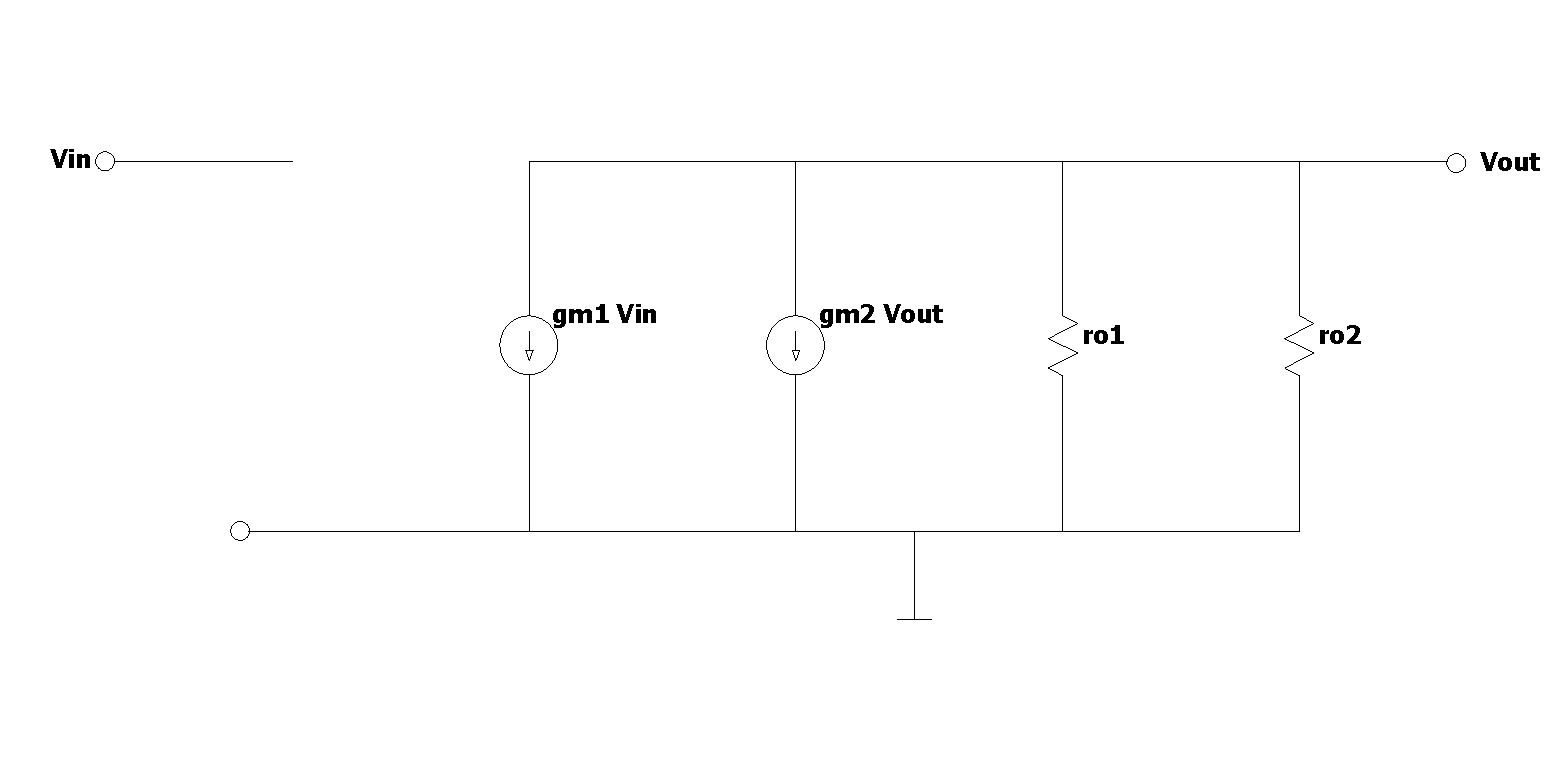
\includegraphics[width=300px]{img/q3/small-signal-model.pdf}
\caption{\label{fig:small-signal-model-q3}Small-signal model of folded-cascode stage}
\end{figure}

\begin{equation*}
\begin{aligned}
R_{out} &= g_{m2}r_{o1}r_{o2} + r_{o1} + r_{o2} \\
&\approx g_{m2}r_{o1}r_{o2}
\\
G_{m} &= \frac{-g_{m1}(g_{m2} + \frac{1}{r_{o1}})}{g_{m2} + \frac{1}{r_{o1}} + \frac{1}{r_{o2}}} \\
&\approx -g_{m1} \\
\\
\frac{V_{out}}{V_{in}} &= g_{m1}g_{m2}r_{o1}r_{o2} \\
\end{aligned}
\end{equation*}
\end{enumerate}
\section{Problem 4}
\label{sec:org7839784}
\begin{enumerate}[(a)]
\item V\textsubscript{out} - V\textsubscript{in} characteristics
\begin{figure}[H]
\centering
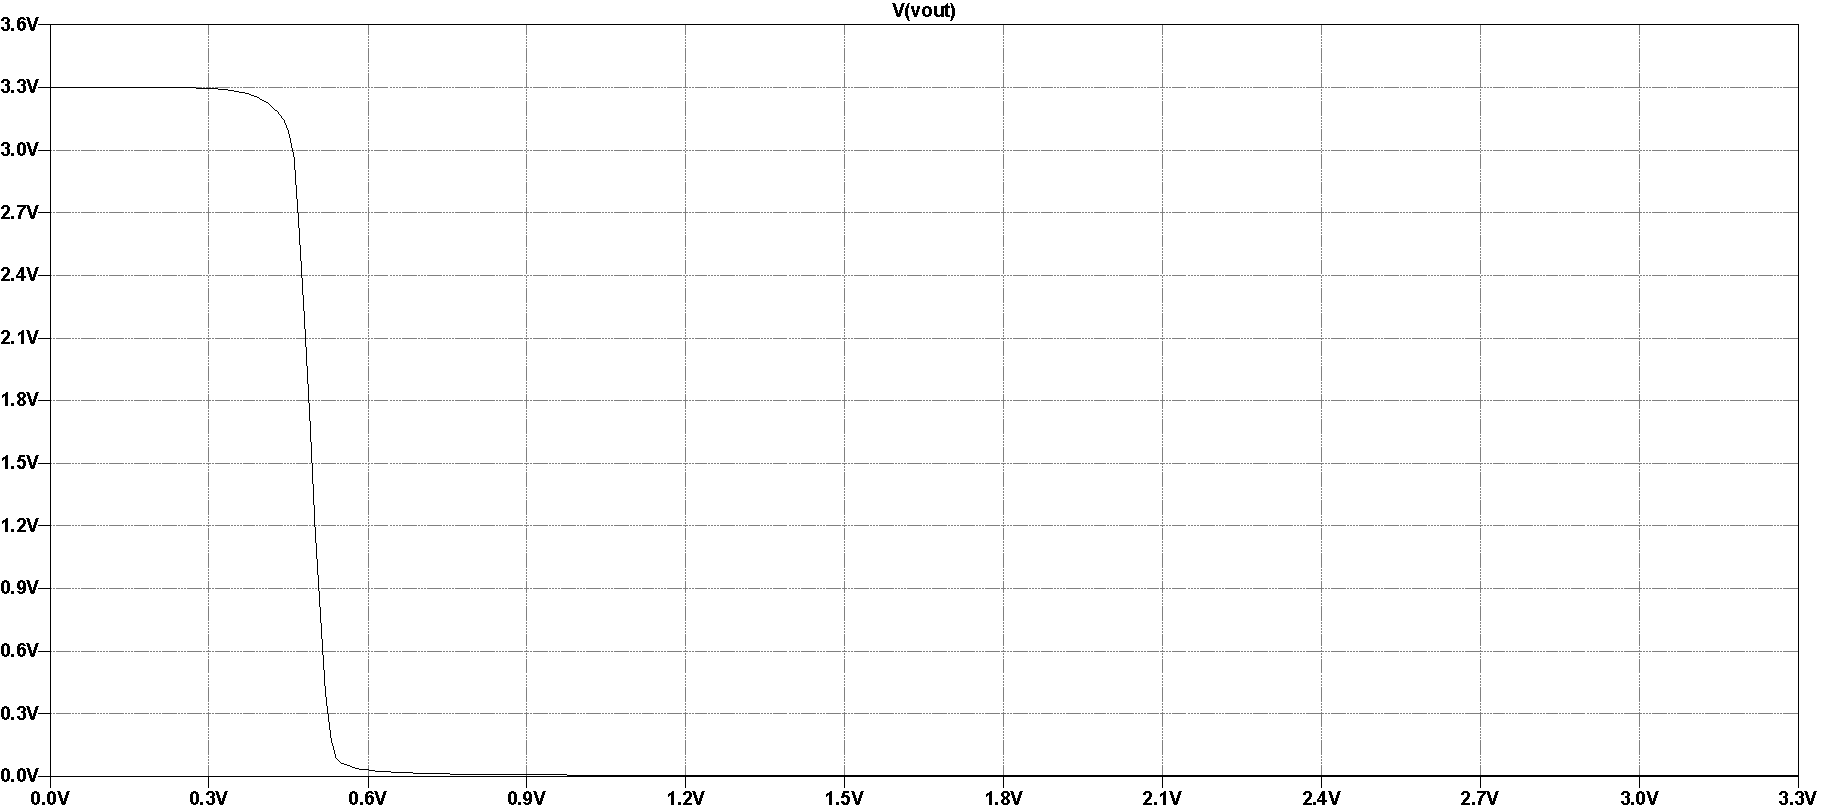
\includegraphics[width=.9\linewidth]{img/q4/a.pdf}
\caption{\label{fig:vout-q4}V\textsubscript{out} - V\textsubscript{in} characteristics}
\end{figure}
\item Small-signal gain, \(\frac{dV_{out}}{dV_{in}}\)
\begin{figure}[H]
\centering
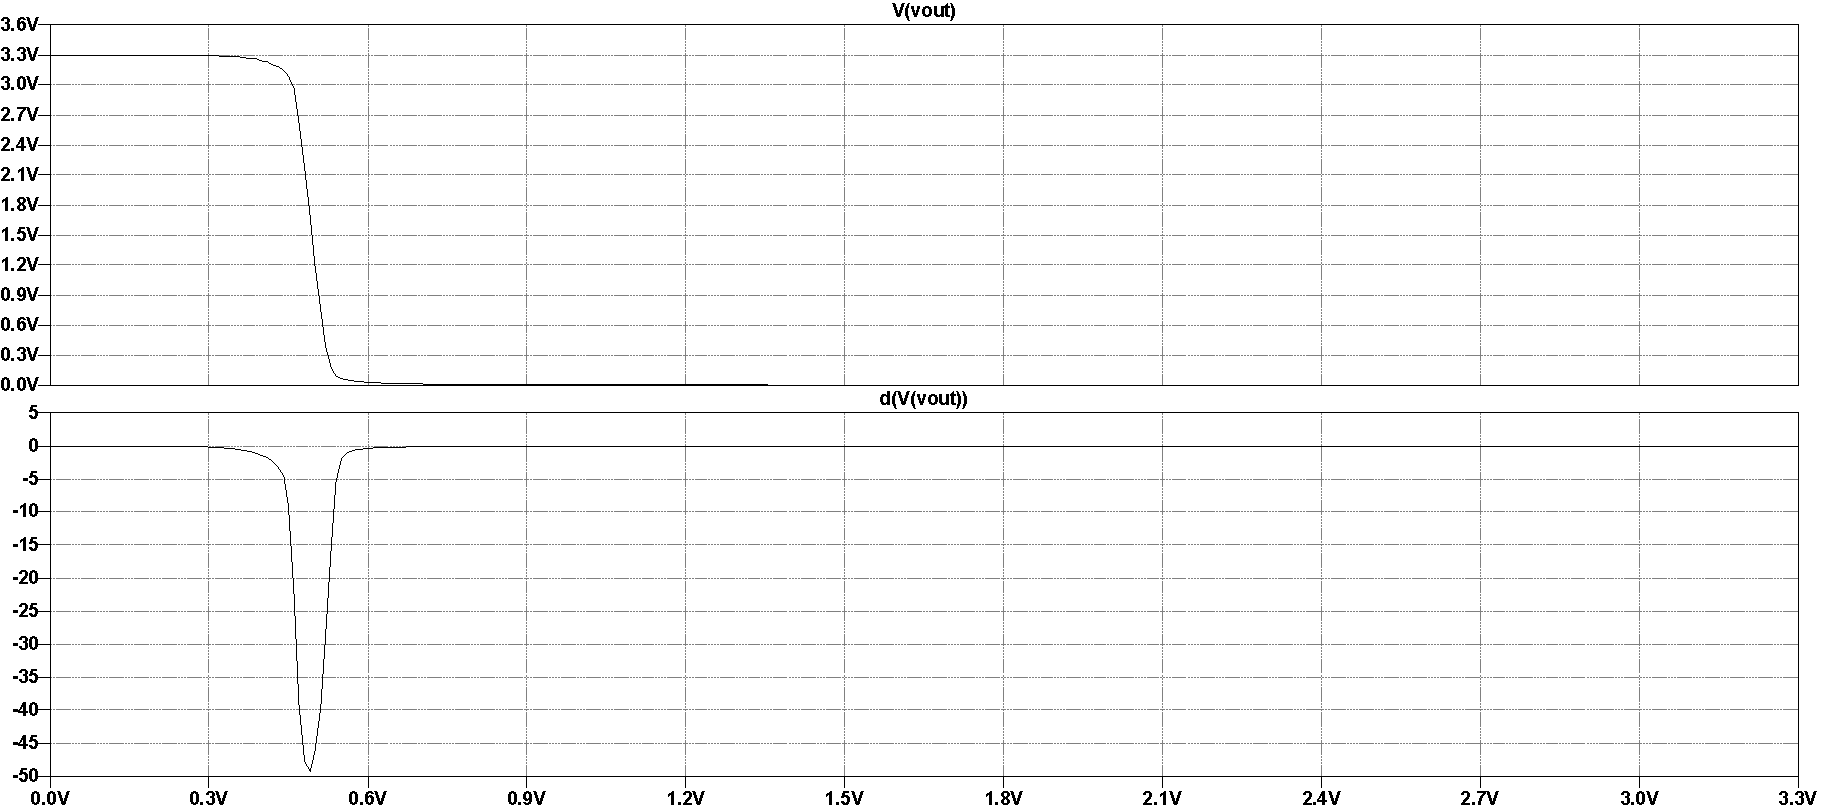
\includegraphics[width=.9\linewidth]{img/q4/b.pdf}
\caption{\label{fig:dvout-q4}Small-signal gain, \(\frac{dV_{out}}{dV_{in}}\)}
\end{figure}

From figure \ref{fig:dvout-q4} the gain when:
\begin{enumerate}[1.]
\item V\textsubscript{out} = 0.6 V

\(\frac{dV_{out}}{dV_{in}} = -35.59\)
\item V\textsubscript{out} = 2.8 V

\(\frac{dV_{out}}{dV_{in}} = -32.77\)
\end{enumerate}
\item From figure \ref{fig:dvout-q4}, the input voltage, V\textsubscript{in}, for maximum gain, \(max(|\frac{dV_{out}}{dV_{in}}|)\) is given to be:
\begin{equation*}
\begin{aligned}
max(|\frac{dV_{out}}{dV_{in}}|) &= 50.07 \\
V_{in} &= 489mV \\
\end{aligned}
\end{equation*}
\item Output voltage swing for gain of 1,
\begin{equation*}
\begin{aligned}
V_{out, max} &= 3.24 V \\
V_{out, min} &= 56 mV \\
V_{out, pp} &= 3.184 V \\
\end{aligned}
\end{equation*}
Output peak to peak voltage
\begin{equation*}
\begin{aligned}
V_{out, pp} &= 3.184 V \\
\end{aligned}
\end{equation*}
\item Small-signal voltage gain when:
\begin{enumerate}[1.]
\item V\textsubscript{out} = 0.6 V, V\textsubscript{in} = 0.514 V
\begin{figure}[H]
\centering
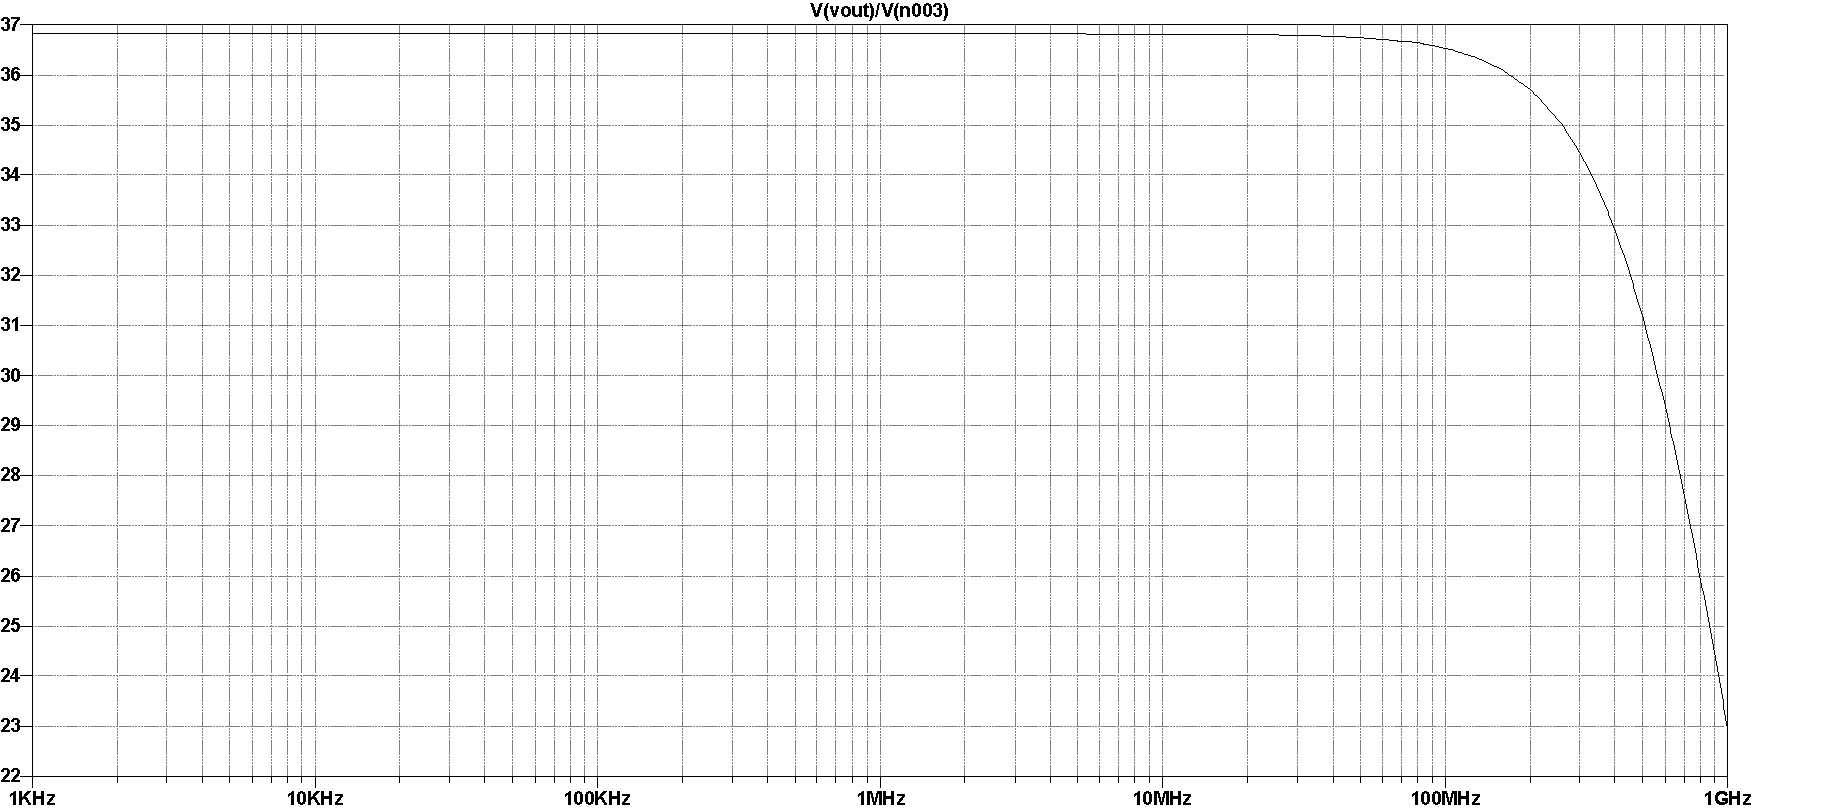
\includegraphics[width=.9\linewidth]{img/q4/e1.pdf}
\caption{\label{fig:gain-q4-e1}Small-signal gain, \(|\frac{V_{out}}{V_{in}}|\), V\textsubscript{out} = 0.6 V, V\textsubscript{in} = 0.514 V}
\end{figure}

Gain = 36.82

\item V\textsubscript{out} = 2.8 V, V\textsubscript{in} = 0.464 V
\begin{figure}[H]
\centering
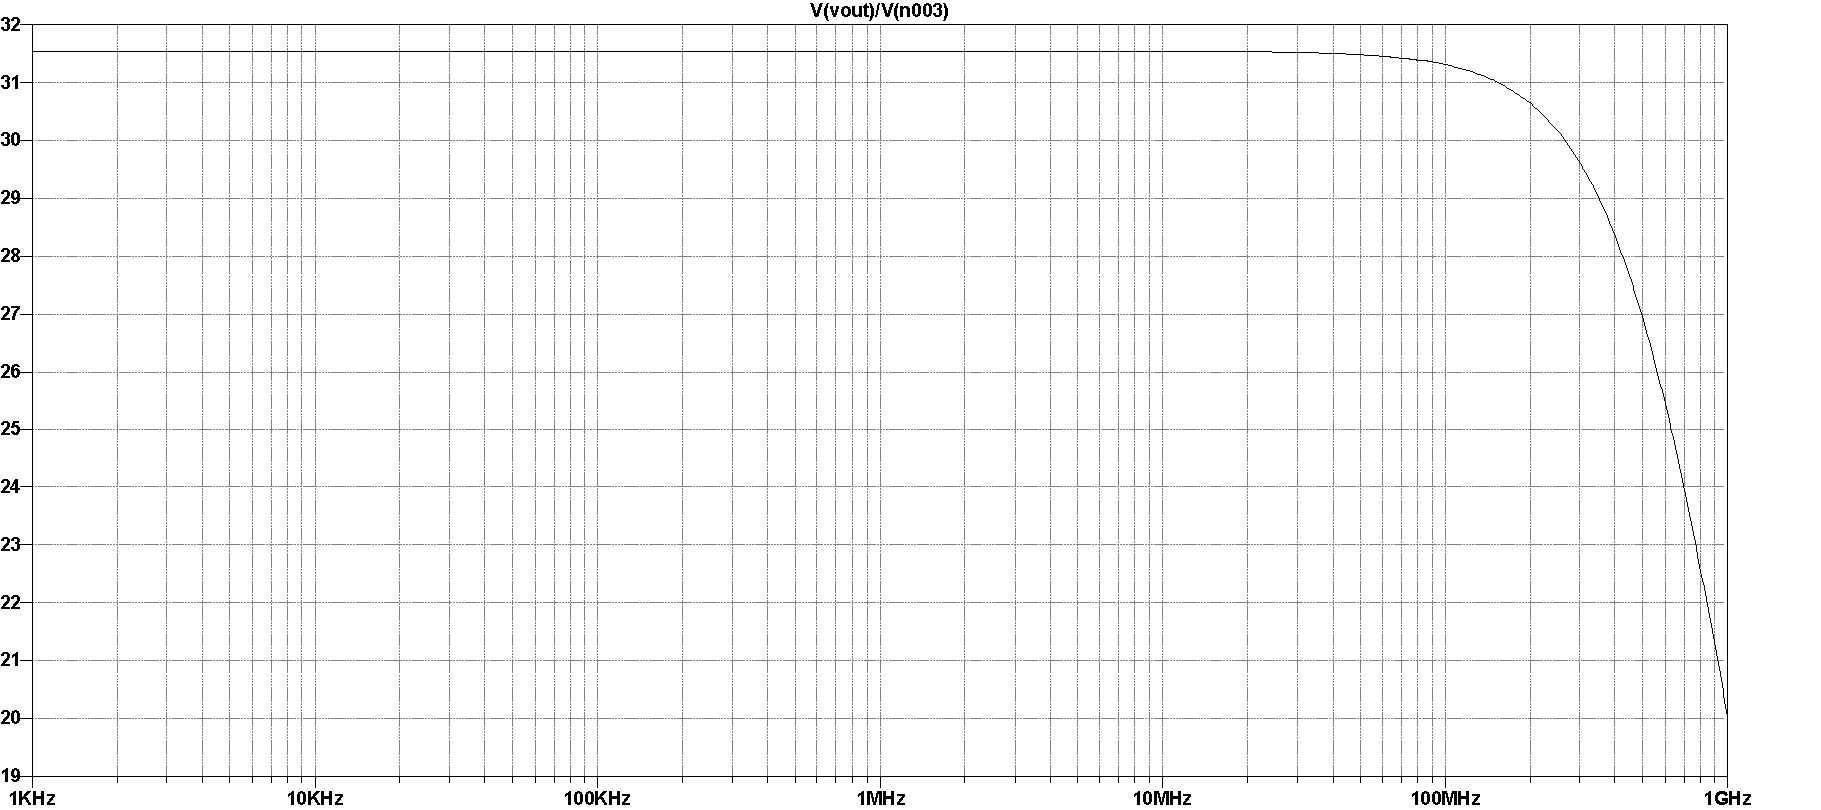
\includegraphics[width=.9\linewidth]{img/q4/e2.pdf}
\caption{\label{fig:gain-q4-e2}Small-signal gain, \(|\frac{V_{out}}{V_{in}}|\), V\textsubscript{out} = 2.8 V, V\textsubscript{in} = 0.464 V}
\end{figure}

Gain = 31.54
\end{enumerate}
\end{enumerate}
\section{Problem 5}
\label{sec:org1ec73a1}
\end{document}
